\begin{figure}
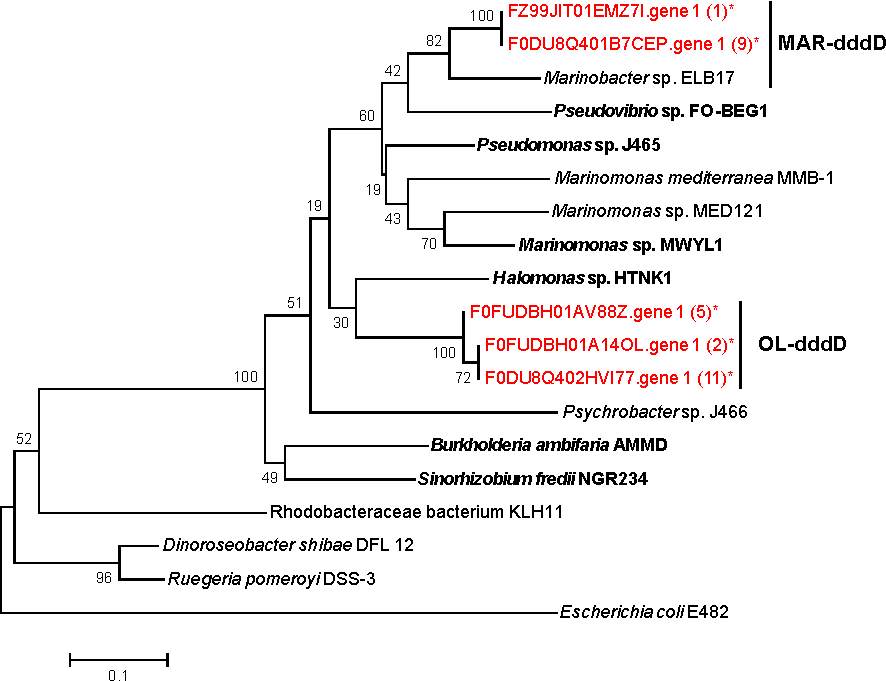
\includegraphics[width=\textwidth]{orglake_figures/dddD_tree.pdf}
\caption[Phylogeny of DddD DMSP lyase homologues]{Phylogeny of DddD DMSP lyase homologues. \emph{E. coli} carnitine coenzyme A transferase was used as an outgroup. \emph{Dinoroseobacter shibae} DFL 12 and \emph{Ruegeria pomeroyi} DSS-3 homologues are a non-functional outgroup \cite{Todd2011}. The tree was computed from a 75 amino acid region within the conserved amino-terminal class III coenzyme A domain (CaiB) using the neighbour-joining algorithm. Organic Lake sequences from this study are shown in red and marked with an asterisk (*). Numbers in parentheses are counts of sequences that clustered with the Organic Lake homologue shown in the tree with 90\% amino acid identity. Sequences with confirmed DMSP lyase activity are shown in bold. Accession numbers from top to bottom are: EBA01716, AEV37420, ACY01992, ADZ91595, EAQ63474, ABR72937, ACV84065, ACY02894, ABI89851, YP\_002822700, EEE36156, ABV95365, AAV94987 and EGB36199.}
\label{fig:dddD_tree}

\end{figure}
